\section{Magnetism}
Where charge ($\vec{E}$-field) has an elementary source unit of a point charge (or monopole) which may be positively or negatively charged. Conversely the elementary source unit of magnetism ($\vec{B}$-field) is the \index{magnetic dipole}. \index{Magnetic monopole}s have never been observed; their existence would also violate Gauss law ($\vec{\nabla} \cdot \vec{B} = 0 $). 
\subsection{Magnetic Dipole}
Classically, the magnetic dipole is though of as a loop carrying an
electric current ($I$). 

The resultant \index{magnetic dipole moment}{magnetic dipole moment}, $\vec{\mu}$, is defined as the vector at a normal to the  
plane of the current loop, 
\begin{equation}
    \vec{\mu} = IS \vec{n}
    \label{eq:dipole_moment}
\end{equation}
where $I$ is the current in, and $S$ the surface area enclosed by, the loop. 

\begin{wrapfigure}{l}{0.4\textwidth}%
    \centering%
    % 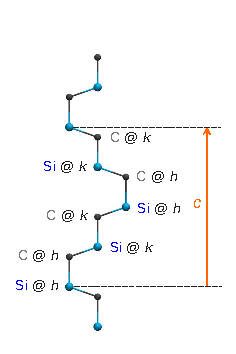
\includegraphics[width=0.38\textwidth]{figures/SiC-non-equiv-sites.pdf}%
        % B FIELD through current loop
\begin{tikzpicture}[scale=1.2, thick]
  \def\Rx{1.45}
  \def\Ry{0.43}
  \def\h{0.5}
  \def\H{3}
  \def\L{4}
  \def\NB{5}
  \def\ang{36}
  \coordinate (O) at (0,0);
  \coordinate (N) at (0,0.24*\H);
  \coordinate (M) at (0,0.45*\H);
  \coordinate (B) at (\ang:\H);
  
  % MAGNETIC FIELD
  \draw (-\Rx,0) arc (180:0:{\Rx} and {\Ry});
  \begin{scope}
    \clip ({-0.5*\L*cos(\ang)},-0.4*\H) rectangle ++({\L*cos(\ang)},\H);
    %\foreach \i [evaluate={\y=(\i-0.5)*\H/(\NB-0.5)/2;
    %                       \yl=-\H/2+(\i-0.5)*\H/(\NB-0.5)/2;}] in {1,...,\NB}{
    %  %\draw[BFieldLine,thin] (0,\y)++(\ang-180:0.5*\L) --++ (\ang:\L);
    %  %\draw[BFieldLine,thin] (0,-\y)++(\ang-180:0.5*\L) --++ (\ang:\L);
    %  \draw[BFieldLine,thin] (-\H/2,\y) -- ({-\H/2+(\H/2-\y)*cos(\ang)},\H/2);
    %  \draw[BFieldLine,thin] (-\H/2,-\y) -- ({-\H/2+(\H/2+\y)*cos(\ang)},+\H/2);
    %  \draw[BFieldLine,thin] ({\H/2-(\H/2+\yl)*cos(\ang)},-\H/2) -- (\H/2,\yl);
    %  \draw[BFieldLine,thin] ({\H/2-(\H/2-\yl)*cos(\ang)},-\H/2) -- (\H/2,-\yl);
    %}
    % \foreach \i [evaluate={\x=-0.31*\H+(\i-1)*0.62*\H/(\NB-1);
    %                        \y=-cot(\ang)*\x;
    %                        \a=0.50+0.017*\i}] in {1,...,\NB}{ %0.58-0.02*(\i-\NB/2-1)^2
    %   \draw[BFieldLine=\a] (\x,\y)++(\ang-180:\H) --++ (\ang:2*\H);
      %\fill[red] (\x,\y) circle (0.05);
    % }
  \end{scope}
  % \node[Bcol] at (\H/2,0.49*\H) {$\vb{B}$};
  
  % CIRCUIT
  \draw[white,very thick]
        (-\Rx,0) arc (-180:0:{\Rx} and {\Ry});
  \draw (-\Rx,0) arc (-180:0:{\Rx} and {\Ry});
  %\draw[white,very thick] (0,0) ellipse ({\R} and {0.3*\R});
  %\draw (0,0) ellipse ({\R} and {0.3*\R});
  %\draw (0,0) ellipse ({\R} and {0.3*\R});
  \draw[mu vector] (0,0) -- (M) node[above=-1, left=0] {$\vb*{\mu}$};
  \draw[vector] (0,0) -- (N) node[below=0,left=0] {$\vu{n}$};
  % \draw pic[->,"\small$\;\theta$",draw=black,angle radius=14,angle eccentricity=1.4]
    % {angle = B--O--N};
  \draw[white,very thick]
    (-150:{1.1*\Rx} and {1.16*\Ry}) arc (-150:-80:{1.1*\Rx} and {1.16*\Ry});
  \draw[current]
    (-135:{1.1*\Rx} and {1.16*\Ry}) arc (-135:-90:{1.1*\Rx} and {1.16*\Ry})
    node[midway,right=2,below] {$I$};
  
\end{tikzpicture}


  \caption{Schematic of current loop and induced magnetic moment.}%
\end{wrapfigure}%


The \index{magnetic dipole}{magnetic dipole} induces a magnetic field $\vec{B}$, which for points a large distance from the dipole may be calculated as \cite{Griffiths2012-pt}:
\begin{equation}
    \vec{B} = \frac{\mu_0}{4\pi} \frac{1}{r^3} \left[\frac{3(\vec{\mu} \cdot \vec{r}) \cdot \vec{r}}{r^2} - \vec{\mu}\right]
    \label{eq:}
\end{equation}

The symmetry of the field enables us to consider the direction of the dipole as aligned to the $z$-axis. Then, defining $x,y$ as usual by $r \cos\theta$ and $r \sin\theta$ respectively. We may decompose the \index{magnetic field}{magnetic field} in two separate components, parallel ($B_z$) and perpendicular ($B_x, B_y$): 
$$B_\parallel =\frac{\mu_0}{r^3}(3\cos^2 \theta - 1), \quad B_\perp = \frac{3\mu_0}{r^3}\cos\theta\sin\theta.$$
Where we use the Pythagorean principle to determine the overall magnitude $B = |\vec{B}|$ as
$$B = \sqrt{B_\parallel^2 + B_\perp^2}.$$

\subsection{Gyromagnetic Ratio}
\subsubsection{Classical Derivation}
The current in equation \ref{eq:dipole_moment} is proportional to the angular momentum of the charge. That is, the dipole moment is always associated with an angular momentum $\vec{G} = \vec{r} \times \vec{p}$ with $\vec{r}$ the radius and $\vec{p}$ the momentum. 

Dividing the magnetic dipole moment by the angular momentum we find the \textbf{gyromagnetic ratio}. 
\begin{equation}
    \gamma = \frac{\vec{\mu}}{\vec{G}}.
    \label{eq:gyromagnetic_ratio}
\end{equation}

Without loss of generality we may consider the most simple case which is where the magnetic dipole moment is parallel (or anti-parallel) to the angular momentum. Then we may consider the absolute values for the dipole moment and the angular momentum: 
\begin{equation}
    \mu = IS, \quad I = 
    % \underbrace{\frac{q}{2\pi R}}_{\rho \text{ (charge density)}}v,
    \frac{qv}{2\pi R},
    \quad S = \pi R^2 
    % \label{eq:}
\end{equation}
We substitute $I$ and $S$ to find 
\begin{equation}
    \mu = \frac{qvR}{2} 
    % \label{eq:}
\end{equation}
% which we substitute into our equation for the gyromagnetic ratio 
% \begin{equation}
%     \gamma = \frac{\frac{qvR}{2}}{\vec{G}}. 
%     \label{eq:789}
% \end{equation}
and further, we equate the angular momentum vector, using the model of a planar loop to 
\begin{equation}
   G= m_q v R 
    % \label{eq:}
\end{equation}
leaving 
\begin{equation}
    \gamma = \frac{q}{2m_q } . 
    % \label{eq:}
\end{equation}

We finally consider that we may represent the, currently unknown, charge and mass as a sum of electron charges and masses. 
\begin{equation}
    \gamma = \frac{q}{2m_q } = \frac{\cancel{N}e}{2\cancel{N} m_e} \implies \gamma = \frac{e}{2 m_e}
    \label{eq:gyromagnetic_ratio}
\end{equation}

We therefore find that the gyromagnetic ratio of the electron depends only on fundamental constants \cite{bromley2000quantum}.

%pg 329 
% https://www.google.co.uk/books/edition/_/7qCMUfwoQcAC?hl=en&gbpv=1&bsq=walter%20greiner%20theoretical%20physics



\subsubsection{Extending to Quantum Mechanics}
Since the gyromagnetic ratio was calculated considering the motion of dipole in a loop, we may extend this to an electron in an orbit.

\begin{wrapfigure}{r}{0.5\textwidth}%
	% \centering%
	\begin{center}
		% 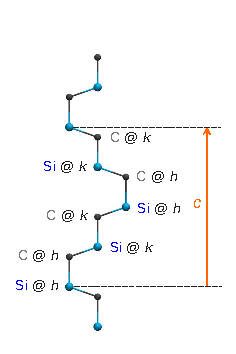
\includegraphics[width=0.38\textwidth]{figures/SiC-non-equiv-sites.pdf}%
		% MAGNETIC MOMENT ATOM
\begin{tikzpicture}[thick, scale=1.5]
  \def\rn{0.3}
  \def\re{0.15}
  \def\Rx{1.5}
  \def\Ry{0.5}
  %\draw[dashed] (-100:1.5*\rn) -- (80:1.5*\rn);
  \draw[dashed] (-\Rx,0) arc (180:0:{\Rx} and {\Ry});
  \draw[mu vector] (0,-1.8*\rn) -- (0,2.9*\rn) node[right] {$\vb*{\mu}$};
  \draw[charge+] (0,0) circle (\rn) node[scale=1.4] {+};
  \draw[dashed] (\Rx,0) arc (0:-180:{\Rx} and {\Ry});
  \draw[charge-]
    (-40:{\Rx} and {\Ry}) circle (\re) node[scale=0.8] {$-$}
    node[below right=0.2] {e};
  \draw[->]
    (-55:{1.15*\Rx} and {1.2*\Ry}) arc (-55:-72:{1.15*\Rx} and {1.2*\Ry});
  \draw[current]
    (-140:{1.15*\Rx} and {1.2*\Ry}) arc (-140:-100:{1.15*\Rx} and {1.2*\Ry})
    node[midway,below] {$I$};
\end{tikzpicture}

		\caption{Schematic of electron in orbit generating a magnetic moment.}%
	\end{center}
\end{wrapfigure}%
The fundamental change required to extend the model to quantum mechanics is the treatment of angular momentum which should now be quantised.
Thus, we replace our classical approximation of $\vec{G} = \vec{r} \times \vec{p}$ with the equation for the eigenvalues of the quantum mechanical representation of orbital angular momentum,
\begin{equation}
	\hat{G} = \hbar \hat{L}
	\label{eq:orbital_angular_momentum}
\end{equation}
where $\hat{L}$ is the operator of the orbital angular momentum (quantum number of orbital momentum).
The angular momentum and total energy are conserved in general in a closed system.

We consider the time independent \index{Shr\"odinger equation}{Shr\"odinger equation}
\begin{equation}
	\hat{H} \Psi_n = E_n \Psi_n
	\label{eq:TISE}
\end{equation}

and choose $\Psi_n$ such that it is an eigenfunction of the Hamiltonian, the total angular momentum squared ($L^2 = L_x^2 + L_y^2 + L_z^2$) and exactly one directional component of the angular momentum which is by convention chosen as $L_z$.

According to quantum mechanics the projection of $L$ along the \index{quantisation axis} ($m_L$) may take integer values $-L, -L + 1, \dots, L-1, L$.
Thus, we may describe a given quantum state by the angular momentum $L$ and it's projection $m_L$. Thus, using \index{Dirac notation}{Dirac Notation} we write
\begin{eqnarray}
	&\hat{H}\ket{L, m_L} &= E\ket{L, m_L} \\
	&\hat{L^2}\ket{L, m_L} &= L(L+1)\ket{L, M_L} \\
	&\hat{L_z}\ket{L, m_L} &= m_L\ket{L, m_L}. \label{eq:zthcomponent}
\end{eqnarray}
Thus, the operator which describes the orbital magnetic moment may be written using  \eqref{eq:gyromagnetic_ratio_electrons}, \eqref{eq:orbital_angular_momentum} as
\begin{equation}
	\hat{\vec{\mu}}_L = \gamma \hat{\vec{G}}_L = \gamma \hbar \hat{\vec{L}} = \frac{e\hbar}{2m_e c}\hat{\vec{L}}.
	\label{eq:orbital_magnetic_moment_operator}
\end{equation}

This leads to a quantity known as the \textbf{\index{Bohr magneton}{Bohr Magneton}}, $\mu_B$, given by \cite{Ramamurti1995-wg}
\begin{equation}
	\mu_B = \frac{|e|\hbar}{2m_e c}.
	\label{eq:bohr_magneton}
\end{equation}

Using this we may write \eqref{eq:orbital_magnetic_moment_operator} as
\begin{equation}
	\hat{\vec{\mu}}_L = -\mu_B\hat{\vec{L}}.
	\label{eq:orbital_magnetic_moment_operator_bohr_magneton}
\end{equation}


\subsection{g-factor}
The above expression is valid for the orbital electron but may be extended to a more general system by introducing a \index{g-factor}{g-factor}. The g-factor is equivalent to a dimensionless gyromagnetic ratio \cite{giancoli2008physics}, so \eqref{eq:orbital_magnetic_moment_operator_bohr_magneton} may be written with $g=1$ as
\begin{equation}
	\hat{\vec{\mu}}_L = -g\mu_B\hat{ \vec{L}}.
	\label{eq:orbital_magnetic_moment_operator_bohr_magneton_g_factor}
\end{equation}




